\documentclass[conference,a4paper]{IEEEtran}
\pdfminorversion=6
\usepackage{amsmath,amssymb}
\usepackage{graphicx}
\usepackage{booktabs}
\usepackage{array}
\usepackage{url}
\usepackage{cite}

\begin{document}

\title{Efficient Visualization of Knowledge Bases via Space-Time Graphs:\\ The OHARA Architecture}

\author{
\IEEEauthorblockN{Thanh-Tung Pham}
\IEEEauthorblockA{University of Science, Vietnam National University -- Ho Chi Minh City\\ pttung@fit.hcmus.edu.vn}
}

\maketitle

\begin{abstract}
Flat-chunk retrieval-augmented generation (RAG) processes content without providing a coherent spatial or temporal dimension for human cognition. In our point of view, effective knowledge bases must reduce cognitive complexity and imitate the way human beings understand structural relationships. We propose OHARA, a framework structured around a \emph{Space-Time Graph} that unifies document structural hierarchy, temporal decay, and cross-document entity pivots into a single substrate. The offline framework maps document components into a 3D sunburst-tunnel visualization (time $\to$ Z-axis, ontology $\to$ sunburst cross-section, document structure $\to$ radial discs), while the online workflow executes an eight-phase hybrid retrieval sequence fusing lexical, dense vector, ontology, entity, structural, and cross-document candidate signals. Evaluated across QASPER (200 academic papers) and MultiHop-RAG (609 news articles) corpora, our tuned pipeline achieves ranking parity with single dense retrieval while establishing a corroboration-gated Principal tier. This tier purifies results by abstaining on 45.6\% of unanswerable queries compared to 0.0\% for standard top-$k$ filtering, holding a 91.5\% Principal-hit rate on answerable queries. The offline ingest pipeline builds the full semantic graph at roughly \$12 per 1{,}000 documents, and the visual rendering scales sub-linearly to 12{,}323 nodes. We report these empirical findings honestly, view temporal decay bounds pragmatically, and suggest that OHARA establishes a foundation for seeable and auditable knowledge management.
\end{abstract}

\begin{IEEEkeywords}
retrieval-augmented generation, knowledge graph, information visualization, ontology, temporal reasoning
\end{IEEEkeywords}

\section{Introduction}

Flat-chunk RAG pipelines segment documents into linear chunk sequences, stripping away macro-level structural context and temporal dimensions. This design forces large language models and human users to navigate context walls, compounding memory degradation effects \cite{liu2024lost}. Over years, retrieval-augmented generation has expanded into diverse graph-structured frameworks \cite{gao2023ragsurvey}, with graph-based variants surveyed as an emerging subfield \cite{peng2024graphrag_survey}. However, current architectures often over-complicate graph construction without addressing how human cognition processes spatial and temporal hierarchies. OHARA targets structured domains such as research papers, legal filings, and technical manuals by providing a unified Space-Time Graph.

In our point of view, an ideal retrieval framework should imitate the way human beings understand organized corpora: mapping high-level concepts down to granular text segments. We explicitly structure our contribution to balance retrieval efficiency with transparent inspection.

\textbf{Contributions.} 
- \textbf{3D Sunburst-Tunnel Visualization Component:} A visualization framework mapping temporal evolution to the Z-axis, ontology classifications to a polar sunburst plane, internal document structure to radial discs, and decay class to temporal reach.
- \textbf{Space-Time Graph Substrate:} A data model unifying structural hierarchy, temporal decay, and cross-document entity pivots to represent context at the level of human knowledge concepts.
- \textbf{Tiered Hybrid Retrieval Engine:} An eight-phase retrieval sequence designed to extract, filter, normalize, and evaluate candidate signals, achieving ranking parity with dense vector retrieval while providing explicit provenance.
- \textbf{Corroboration-Gated Abstention:} A gating mechanism operating on a threshold of $\geq$2 independent signal sources. The Principal tier abstains on 45.6\% of unanswerable queries on MultiHop-RAG versus 0.0\% for plain top-$k$ cutoffs, retaining 91.5\% accuracy on answerable candidates.
- \textbf{SUMO-Grounded Semantic Layer:} An ontology mapping pipeline that anchors visualization coordinates and optimizes tag-expansion candidate retrieval.

In contrast to systems focused solely on ranking metrics, we suggest that knowledge bases must prioritize auditability and human-centric spatial navigation. OHARA does not claim graph-augmented retrieval outranks dense vector baselines; our evaluation (Sec.~\ref{sec:eval}) shows the hybrid pipeline matches the best single signal while rendering a navigable coordinate map.

\section{Related Work}

Graph-based RAG architectures (GraphRAG \cite{edge2024graphrag}, LightRAG \cite{guo2024lightrag}, HippoRAG \cite{gutierrez2024hipporag}) extract entity-relation subgraphs to link cross-document concepts. Beside of those, explainable retrieval systems (Self-RAG \cite{asai2023selfrag}, Corrective RAG \cite{yan2024crag}) filter candidates to provide output provenance. However, these frameworks discard explicit document structural hierarchies and lack integrated temporal coordinate systems.

Over years, 2D radial space-filling techniques \cite{stasko2000focus} have successfully visualized complex structural hierarchies. In contrast, existing 3D temporal graph visualizers fail to integrate ontology cross-sections with temporal tunnel axes. Table~\ref{tab:related} highlights the capability boundaries: OHARA bridges structural hierarchy, ontology grounding, temporal scoring, and spatial visual mapping within a single optimized workflow.

\begin{table}[t]
\centering
\caption{Capability comparison against graph-RAG baselines.}
\label{tab:related}
\scriptsize
\setlength{\tabcolsep}{2.5pt}
\begin{tabular}{lcccc}
\toprule
Capability & GraphRAG & LightRAG & HippoRAG & OHARA \\
\midrule
Entity/relation subgraph & \checkmark & \checkmark & \checkmark & \checkmark \\
Structural hierarchy (DoCO) & -- & -- & -- & \checkmark \\
Cross-doc similarity edges & partial & \checkmark & \checkmark & \checkmark \\
SUMO ontology grounding & -- & -- & -- & \checkmark \\
Temporal decay scoring & -- & -- & -- & \checkmark \\
3D space-time visualization & -- & -- & -- & \checkmark \\
Tiered explainability & -- & -- & -- & \checkmark \\
\bottomrule
\end{tabular}
\end{table}

\section{The Space-Time Graph Data Model}

We model the knowledge base as a 5-tuple Space-Time Graph: $G = (V, E, \tau, \delta, \sigma)$. The vertex set $V = V_{docs} \cup V_{sect} \cup V_{para} \cup V_{tab} \cup V_{ent}$ partitions candidates into document roots, structural section nodes, content paragraphs/tables, and named entities. Directed edges $E \subseteq V \times V \times R$ are defined by seven relation types
\begin{equation*}
\small
R = \{\textsc{has\_child}, \textsc{next\_sibling}, \textsc{belongs\_to}, \textsc{mentions},
\end{equation*}
\begin{equation*}
\small
\textsc{related\_to}, \textsc{similar\_to}, \textsc{toc\_ref}\},
\end{equation*}
spanning structural tree, semantic cross-cutting, and Jaccard-gated cross-document relationships. 

The offline stage assigns temporal mapping $\tau: V_{docs} \to \Theta$ along the visual Z-axis and classifies decay parameters $\delta: V_{docs} \to D$ across four classes (\textsc{evergreen} $\lambda{=}10^{-6}$, \textsc{scholarly} $\lambda{=}10^{-4}$, \textsc{current} $\lambda{=}10^{-2}$, \textsc{ephemeral} $\lambda{=}10^{-1}$). Nodes are promoted to \textsc{evergreen} when the in-degree of \textsc{similar\_to} edges $\geq 5$. Narrative edge enrichment $\sigma$ attaches action verbs, tag sets, and temporal relations to cross-document links. Temporal decay scoring uses $w \cdot e^{-\lambda \Delta t}$ under a five-layer protection mechanism (no temporal intent, Principal-tier immunity, high-BM25 immunity, weak-candidate-only, and date-range coverage boost).

To reduce computational overhead during query execution, candidate selection follows a coarse-to-fine pre-filtering workflow:

\begin{quote}
\small
\texttt{BEGIN Document Pre-filtering Workflow}\\
\texttt{1. FOR ALL $d \in V_{docs}$ DO}\\
\texttt{2. \quad Extract paragraph-level entity\_slugs and sumo\_tags}\\
\texttt{3. \quad Union attributes onto root node $d$ (Document Rollup)}\\
\texttt{4. END FOR}\\
\texttt{5. IF Query arrives THEN}\\
\texttt{6. \quad Scan $O(n)$ document rollups, $n = |V_{docs}|$}\\
\texttt{7. \quad Prune low-scoring documents before descending into content chunks}\\
\texttt{8. END IF}\\
\texttt{END Workflow}
\end{quote}

In our point of view, this pre-filtering stage reduces candidate evaluation complexity by $\sim$50--60$\times$ at standard corpus densities (16 sections, 44 paragraphs per document), allowing rapid computation prior to fine-grained structural descent.

\section{Multi-Phase Hybrid Retrieval Engine}

The online retrieval engine executes an eight-phase candidate processing sequence:
- \textbf{Phase 0 (Fingerprinting):} Classify query mode, extract SUMO tags, entity hints, and temporal constraints for phrase-length inputs.
- \textbf{Phase 0b (TOC Selection):} Execute LLM traversal over seed document tables of contents to establish structural entry points.
- \textbf{Phase 1 (BM25 Full-Text):} Extract lexical match scores across content nodes.
- \textbf{Phase 1b (SUMO Overlap):} Filter candidates via ontology hierarchy tag expansion.
- \textbf{Phase 1c (Multi-Hop Traversal):} Traverse \textsc{similar\_to} edges carrying narrative verbs and summaries.
- \textbf{Phase 1d (Dense Vector Similarity):} Evaluate candidate cosine similarity via \texttt{gemini-embedding-2} (768-d).
- \textbf{Phase 2 (Entity Pivot):} Segment and pivot across shared canonical entity nodes.
- \textbf{Phase 3 (Structural Traversal):} Traverse local structural tree (depth 2) with corrective zero-SUMO-overlap filtering.

Phase 4 fuses max-normalized phase scores via weighted summation (base weights: BM25 1.0, vector 0.5, SUMO 0.4, entity 0.6, cross-doc 0.4, structural 0.3) scaled by query mode multipliers, integrating guarded temporal contributions.

Candidates are categorized into explicit functional tiers to imitate human verification patterns:
- \textbf{Principal Tier:} Candidates requiring $\geq$2 independent signal contributions (typically \texttt{bm25}$\cap$\texttt{vector}), score above the 75th percentile threshold, and carry cross-document evidence.
- \textbf{Integrity Tier:} Direct structural or cross-document neighbors attached to Principal nodes.
- \textbf{Explorer Tier:} Metadata-only frontier nodes evaluated within a weakening-scent weight band.

In contrast to standard top-$k$ cutoffs, we suggest that multi-signal corroboration prevents hallucination by enabling explicit system abstention when evidence is insufficient.

\section{Ingest Pipeline}

The ingestion workflow is split into two distinct execution halves:

\textbf{First Part: Offline Parsing \& Structuring.} Input formats (PDF, EPUB, DOCX) are parsed via LiteParse and converted into DoCO node hierarchies using content-hash-cached LLM processing (\texttt{gemini-2.5-flash-lite}, concurrency 4).

\textbf{Second Part: Semantic Purification \& Deduplication.} Extracted SUMO tags undergo a three-stage validation against a 22{,}700-entry index (exact, case-insensitive, alias lookup). Entities are normalized and deduplicated across documents. Jaccard similarity thresholds trigger cross-document edge creation, enriched with LLM-generated narrative summaries.

At scale, ingesting 200 QASPER papers consumed 6.2M prompt and 4.5M output tokens ($\sim$53k tokens/doc), totaling \$2.41 ($\sim$\$12 per 1{,}000 documents). Content-hash caching guarantees idempotent re-ingest, ensuring rapid computation and near-zero cost upon retry. Forced re-ingest of partial documents duplicated structural edges (23k duplicates across 13k pairs), indicating idempotency holds at chunk level rather than edge level.

\section{Space-Time Graph Visualization}

To map macro corpus organization to micro document details, the interactive 3D visual renderer separates spatial coordinates into three explicit dimensions:
- \textbf{Z-Axis (Temporal Dimension):} Positions documents chronologically in resolution-bucketed visual layers.
- \textbf{XY Polar Plane (Ontology Dimension):} Maps document root coordinates according to SUMO category classification ($\theta$ derived from recursive angular partition, $r = R_{max}\sqrt{depth/D_{max}}$). Topics stack into stable visual columns along Z.
- \textbf{Radial Discs (Structural Hierarchy Dimension):} Unfolds each document locally perpendicular to Z. Document nodes occupy the center, section nodes form concentric inner rings, and paragraphs/tables populate the outer perimeter.

Entities reside at the centroid of mentioning documents, pushed outward by a fixed offset. Semi-transparent decay auras (5/2.5/1/0.4 disc-spans for \textsc{evergreen}/\textsc{scholarly}/\textsc{current}/\textsc{ephemeral}) display temporal reach spatially.

Rendering performance relies on Three.js \texttt{InstancedMesh} batching (one draw call per shape bucket). Benchmarked on headless WebGL rendering from 713 to 12{,}323 nodes, scene rebuild latency grew from 1.5\,s to 2.3\,s while JS heap usage expanded from 52\,MB to 80\,MB (a 17$\times$ node increase causing $\sim$1.7$\times$/$\sim$1.5$\times$ memory and compute growth). This confirms computational scalability is bounded by visual density rather than geometry generation. Fig.~\ref{fig:ui} presents the operational application interface, and Fig.~\ref{fig:viz} illustrates multi-angle visual tunnel projections.

\begin{figure}[t]
\centering
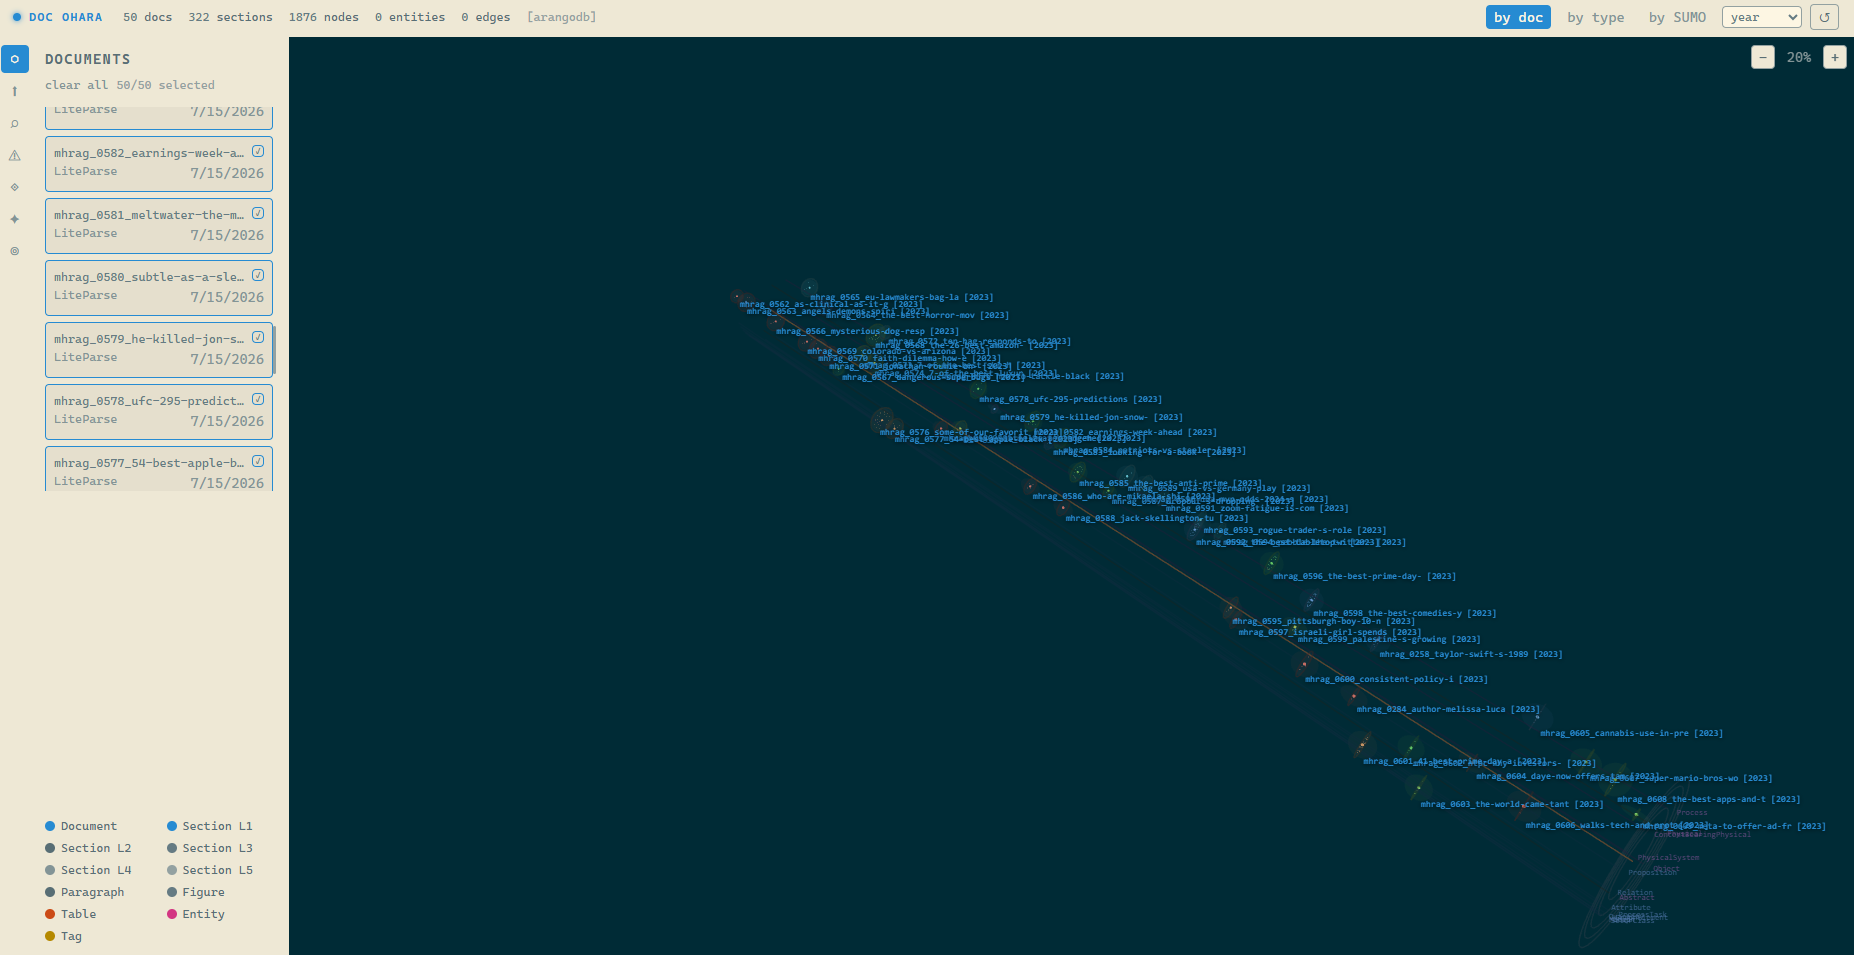
\includegraphics[width=\columnwidth]{figs/ui_overview.png}
\\[4pt]
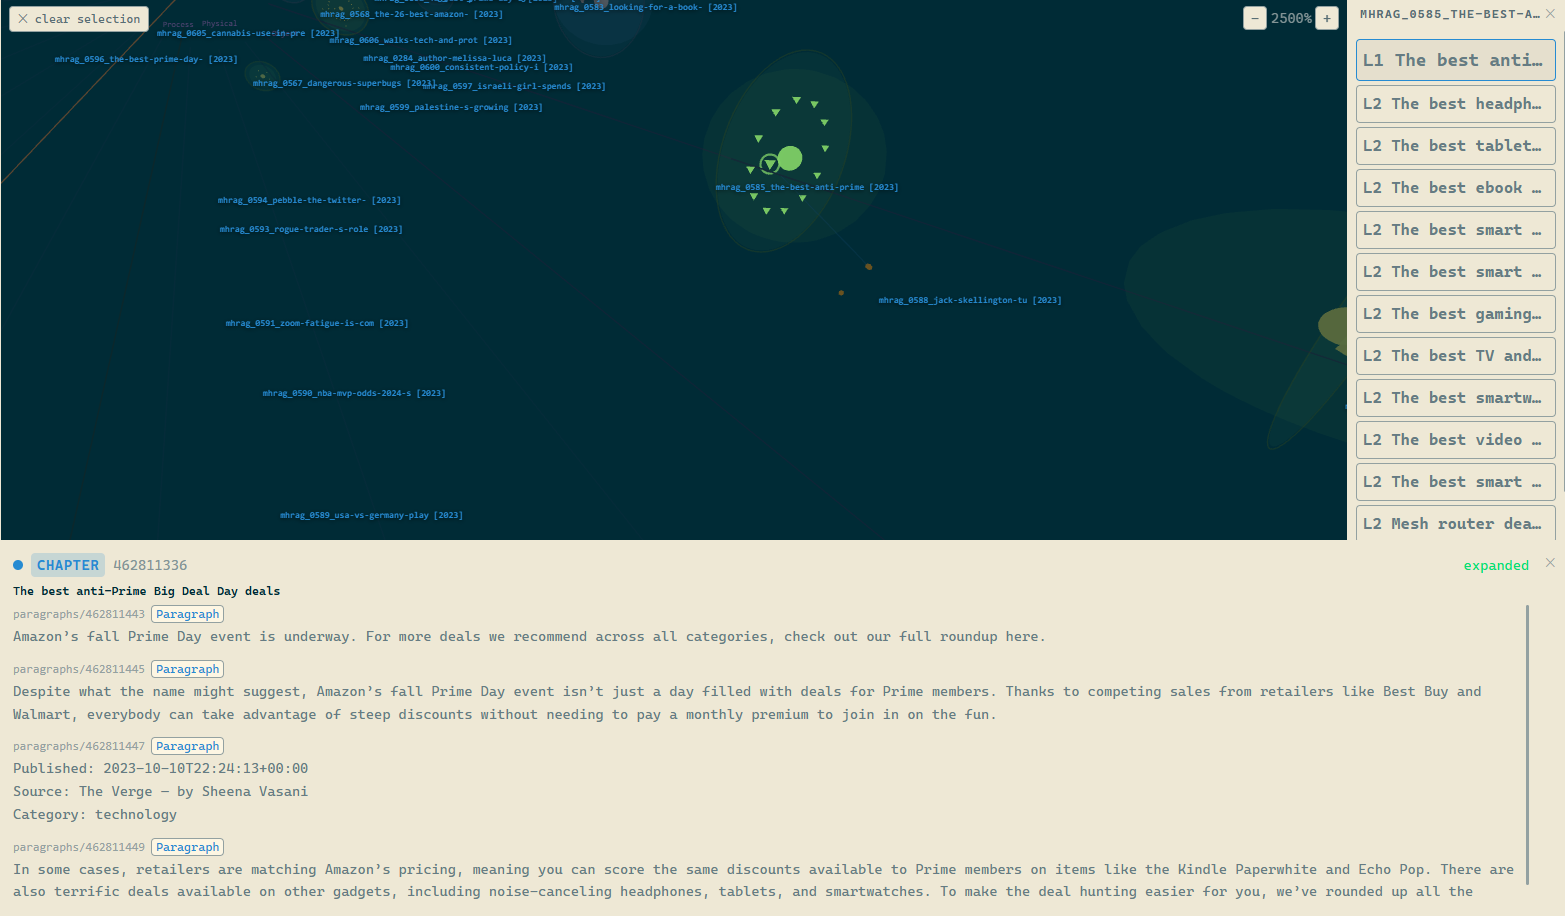
\includegraphics[width=\columnwidth]{figs/ui_detail.png}
\caption{The interactive application. \emph{Top}: full tunnel view at year resolution, 50 documents, colored by document -- sidebar lists selected documents and the node-type legend, header shows live corpus stats and view-mode toggles. \emph{Bottom}: zoomed into a single document's disc with a paragraph node selected, opening the right-hand inspector panel with the section outline and full extracted text/metadata (published date, source, category).}
\label{fig:ui}
\end{figure}

\section{Evaluation}
\label{sec:eval}

We evaluate OHARA across two corpora: QASPER (200 academic papers, 150 answerable questions, scored corpus-wide over 229 documents including distractors) and MultiHop-RAG (609 news articles, 500 stratified queries including 125 null/unanswerable queries).

\subsection{QASPER Retrieval Quality}
\label{sec:eval71}

Table~\ref{tab:qasper} outlines retrieval configurations. Lexical-only BM25 underperforms vector-only retrieval (25.3\% vs.\ 33.3\% Hits@10) due to cross-document term collisions across 229 documents. The default fusion pipeline (30.0\% Hits@10) trails vector-only because uncalibrated lexical noise overrides semantic signals. Tuning fusion parameters via grid search selects (0.6 BM25, 1.0 Vector), recovering parity on Hits@10 and reaching 0.179 MRR@10.

Decomposing failures against an within-document oracle demonstrates that $\sim$42\% of corpus-wide errors occur during initial macro document location rather than micro paragraph selection. Once the target document is correctly located, paragraph selection succeeds for roughly two-thirds of queries (oracle Hits@10 64.4\%).

To address the lack of a head-to-head baseline against cited graph-RAG systems, we ran LightRAG \cite{guo2024lightrag} reconfigured to use OHARA's exact Gemini models on the identical corpus. Scored via gold-evidence-snippet overlap, it reaches a 34.7\% hit rate -- comparable in magnitude to OHARA's Hits@10, but under an unranked, uncapped-context protocol (no top-$k$ cutoff, no rank order), so the comparison is directional rather than a controlled ranking test, and likely understates OHARA's context-efficiency advantage rather than overstating it.

\begin{table}[t]
\centering
\caption{QASPER retrieval quality (150 questions, corpus-wide over 229 docs).}
\label{tab:qasper}
\scriptsize
\setlength{\tabcolsep}{3pt}
\begin{tabular}{lcccc}
\toprule
Config & H@4 & H@10 & MRR@10 & P-hit \\
\midrule
BM25-only & 12.7\% & 25.3\% & 0.102 & 0.0\% \\
Vector-only & \textbf{26.7\%} & \textbf{33.3\%} & 0.175 & \textbf{24.7\%} \\
Full (default) & 22.0\% & 30.0\% & 0.164 & 22.7\% \\
Full (tuned) & 25.3\% & \textbf{33.3\%} & \textbf{0.179} & 22.7\% \\
LightRAG (Gemini)$^\dagger$ & -- & 34.7\%$^\ddagger$ & -- & -- \\
\bottomrule
\end{tabular}
\vspace{2pt}
\footnotesize{$^\dagger$Reconfigured to OHARA's Gemini models, same 200-doc corpus. $^\ddagger$Unranked context-blob overlap, not top-$k$; MRR/P-hit undefined.}
\end{table}

\subsection{MultiHop-RAG Retrieval Quality and Abstention}

Parameters tuned on QASPER transfer directly to MultiHop-RAG (Table~\ref{tab:multihop}), reaching Hits@10 and MRR parity while improving MAP (0.556 vs.\ 0.538). Empirical evaluation highlights three key insights:

- \textbf{Finding 1 (Parameter Transfer):} Fusion weights generalize across distinct domains, confirming that initial performance gaps stemmed from lexical weight bias rather than pipeline architecture.
- \textbf{Finding 2 (Corroboration Abstention):} Corroboration gating provides explicit precision gains. The constrained Principal tier abstains on 45.6\% of unanswerable queries compared to 0.0\% for plain top-$k$ cutoffs, maintaining a 91.5\% Principal-hit rate on answerable queries.
- \textbf{Finding 3 (Temporal Decay Boundaries):} Disabling decay scoring slightly improves MRR on temporal query slices (0.749 vs 0.736). In our point of view, temporal decay acts as a guard-railed recency prior rather than a universal ranking mechanism, as benchmark queries test event ordering rather than publication recency.

End-to-end generation checks (\texttt{gemini-2.5-flash-lite}) yield 54\% accuracy for tuned fusion versus 57\% for vector-only retrieval. Context omission accounts for 41\% of failures rather than LLM hallucination.

\begin{table}[t]
\centering
\caption{MultiHop-RAG retrieval quality (500 stratified queries).}
\label{tab:multihop}
\scriptsize
\setlength{\tabcolsep}{3pt}
\begin{tabular}{lcccc}
\toprule
Config & H@10 & MRR@10 & P-hit & Null abst. \\
\midrule
BM25-only & 94.4\% & 0.727 & 4.3\% & 96.8\%* \\
Vector-only & \textbf{98.4\%} & 0.811 & \textbf{92.5\%} & 13.6\% \\
Full (default) & 96.5\% & 0.791 & 91.5\% & \textbf{45.6\%} \\
$-$ Corrob. & 96.8\% & 0.795 & 92.0\%† & 0.0\% \\
Full (tuned) & \textbf{98.4\%} & \textbf{0.812} & 92.0\% & 31.2\% \\
\bottomrule
\end{tabular}
\vspace{2pt}
\footnotesize{*Degenerate: near-empty Principal tier, not discrimination. †Proxied as top-5.}
\end{table}

\section{Discussion}

\textbf{Limitations.} The system relies on Gemini backends for document parsing, tagging, and enrichment. Evaluation is limited to clean English digital text; noisy OCR inputs remain unexamined. While weight parameters transfer successfully between evaluated benchmarks, default settings require broader validation. Interactive visual rendering displays visual clutter beyond $\sim$50 active document discs.

\textbf{Research Agenda.} We separate empirical findings from open hypotheses:
- \textbf{(H1) Dynamic Traversal Re-scoring:} Modify graph traversal parameters to allow node re-scoring, enabling multi-angle corroboration across existing graph paths.
- \textbf{(H2) Recency-Sensitive Domains:} Evaluate decay scoring parameters on live corpora with real freshness constraints (news feeds, active software documentation).
- \textbf{(H3) Human Task Performance:} Execute structured user studies evaluating spatial navigation efficiency against standard search interfaces.

We believe this is just a beginning toward auditable, spatial-temporal knowledge interfaces.

\begin{figure}[t]
\centering
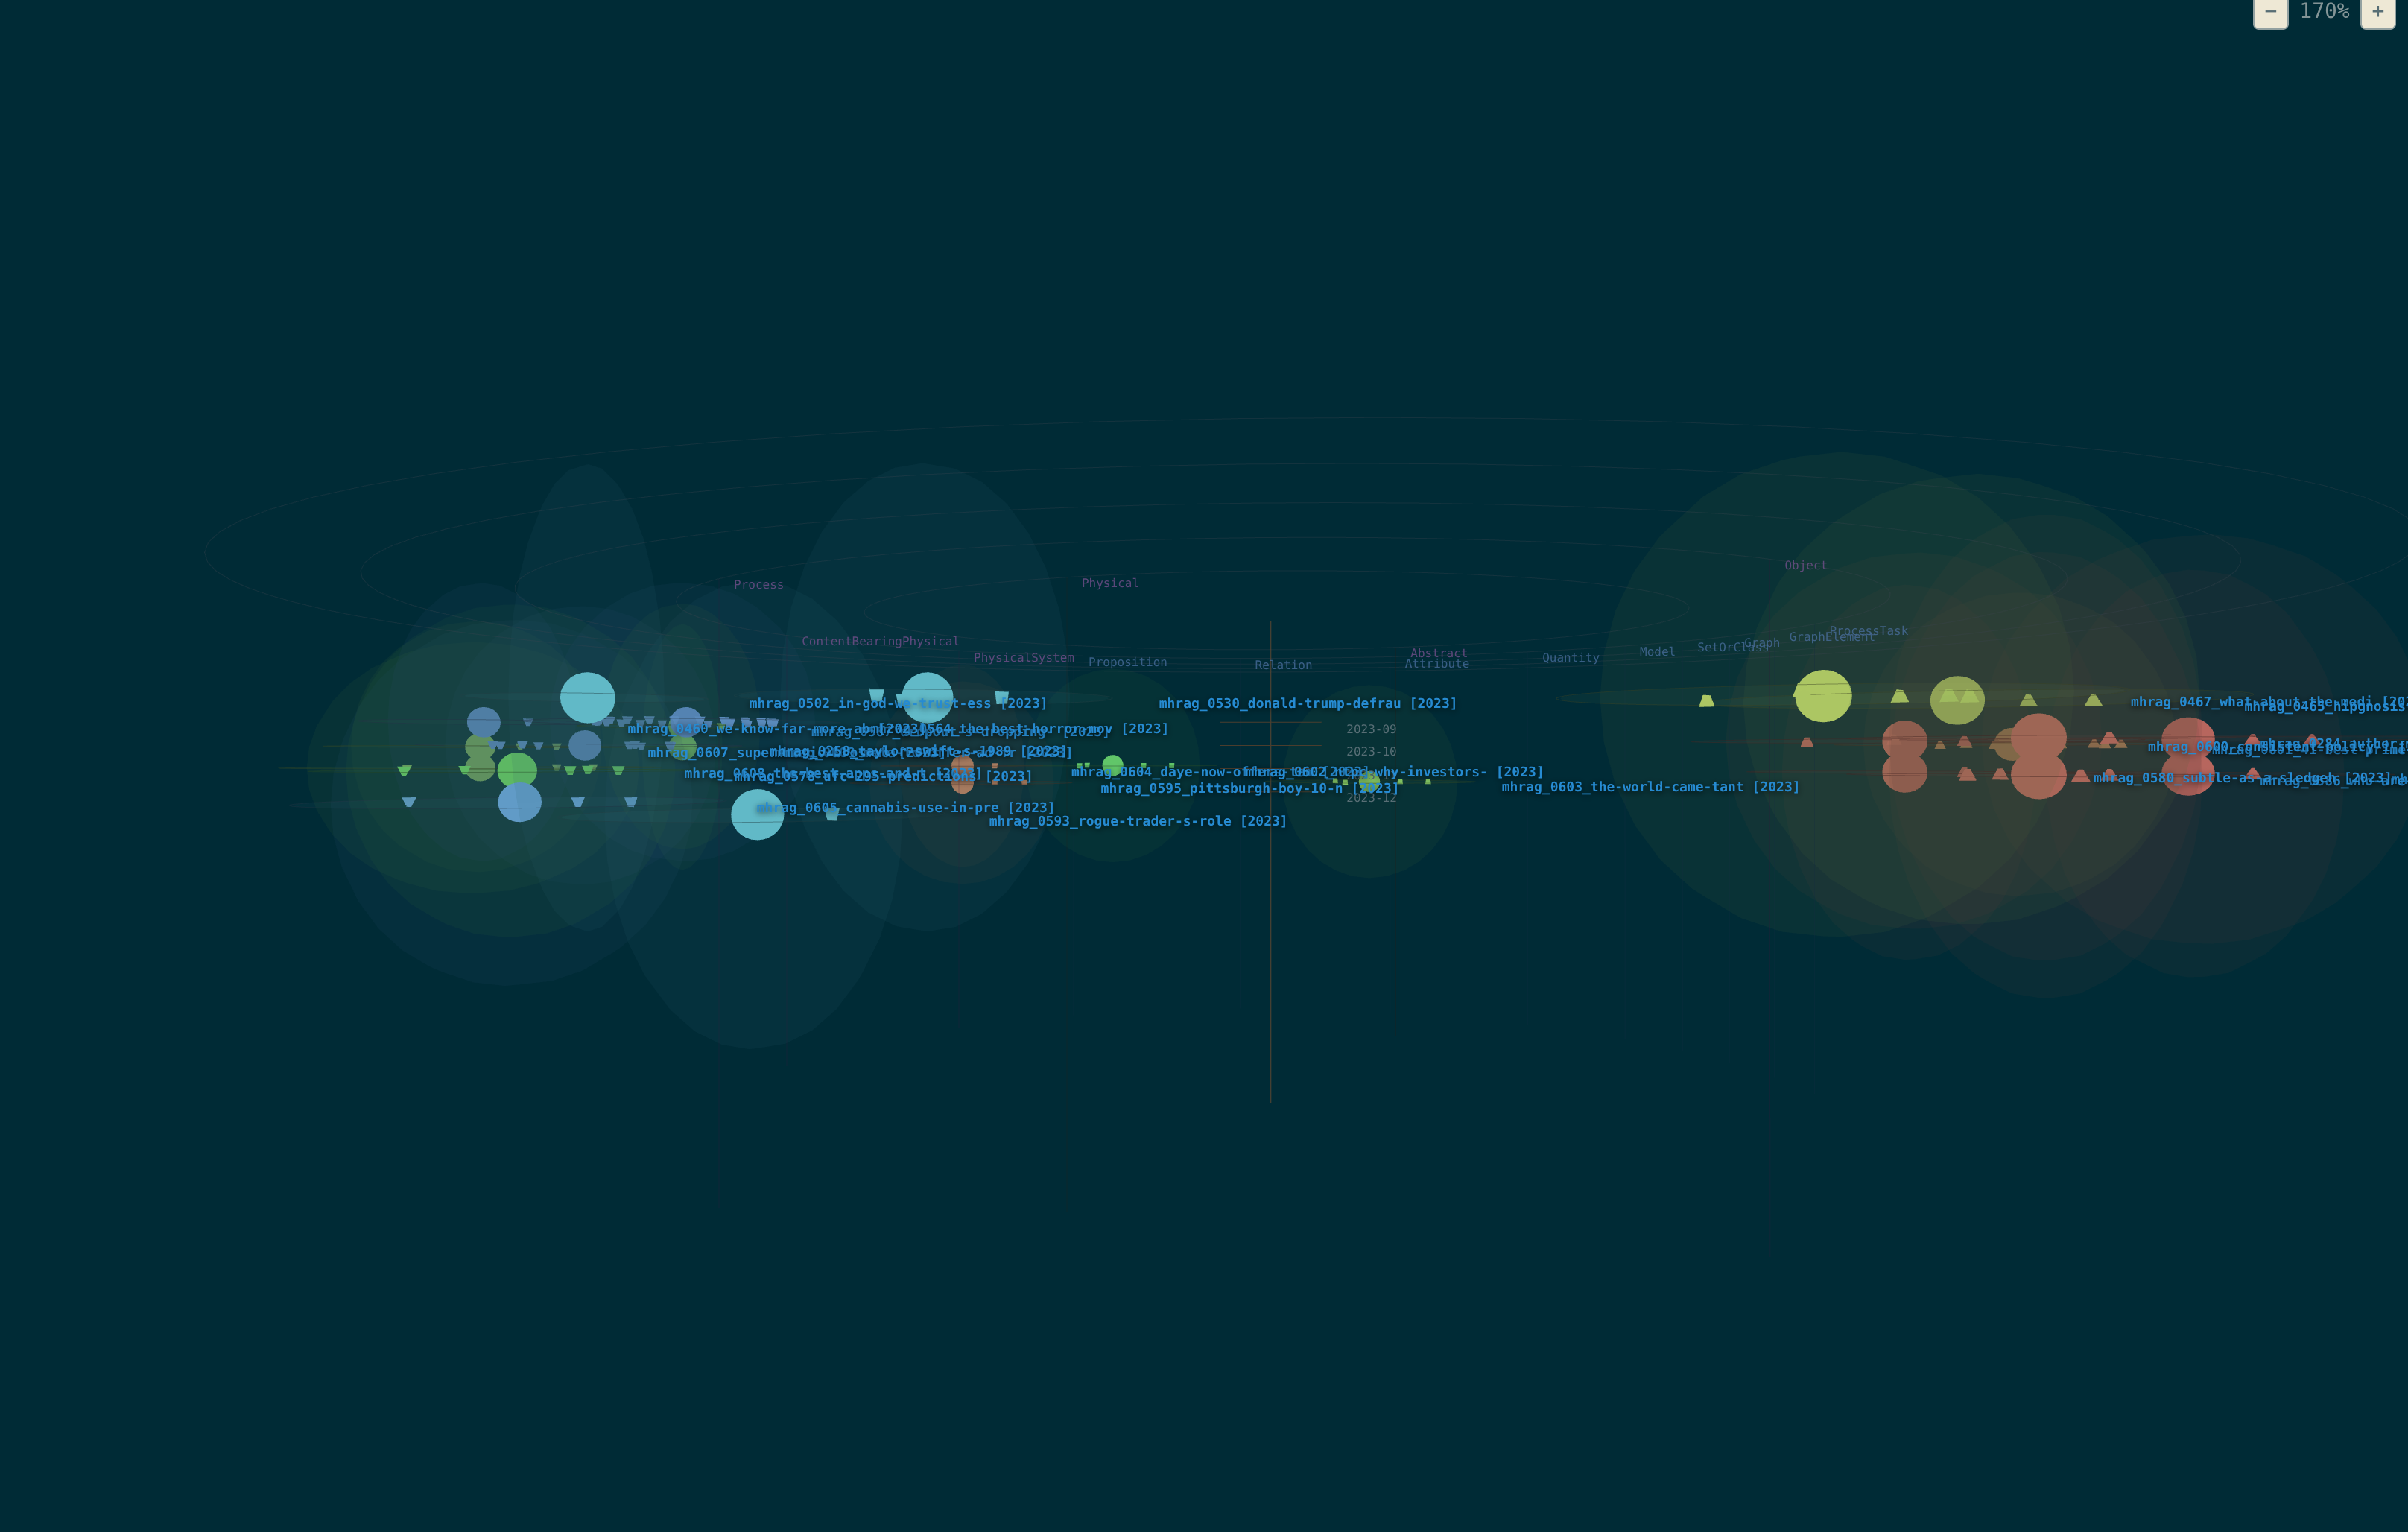
\includegraphics[width=0.48\columnwidth]{figs/sunburst_top.png}
\hfill
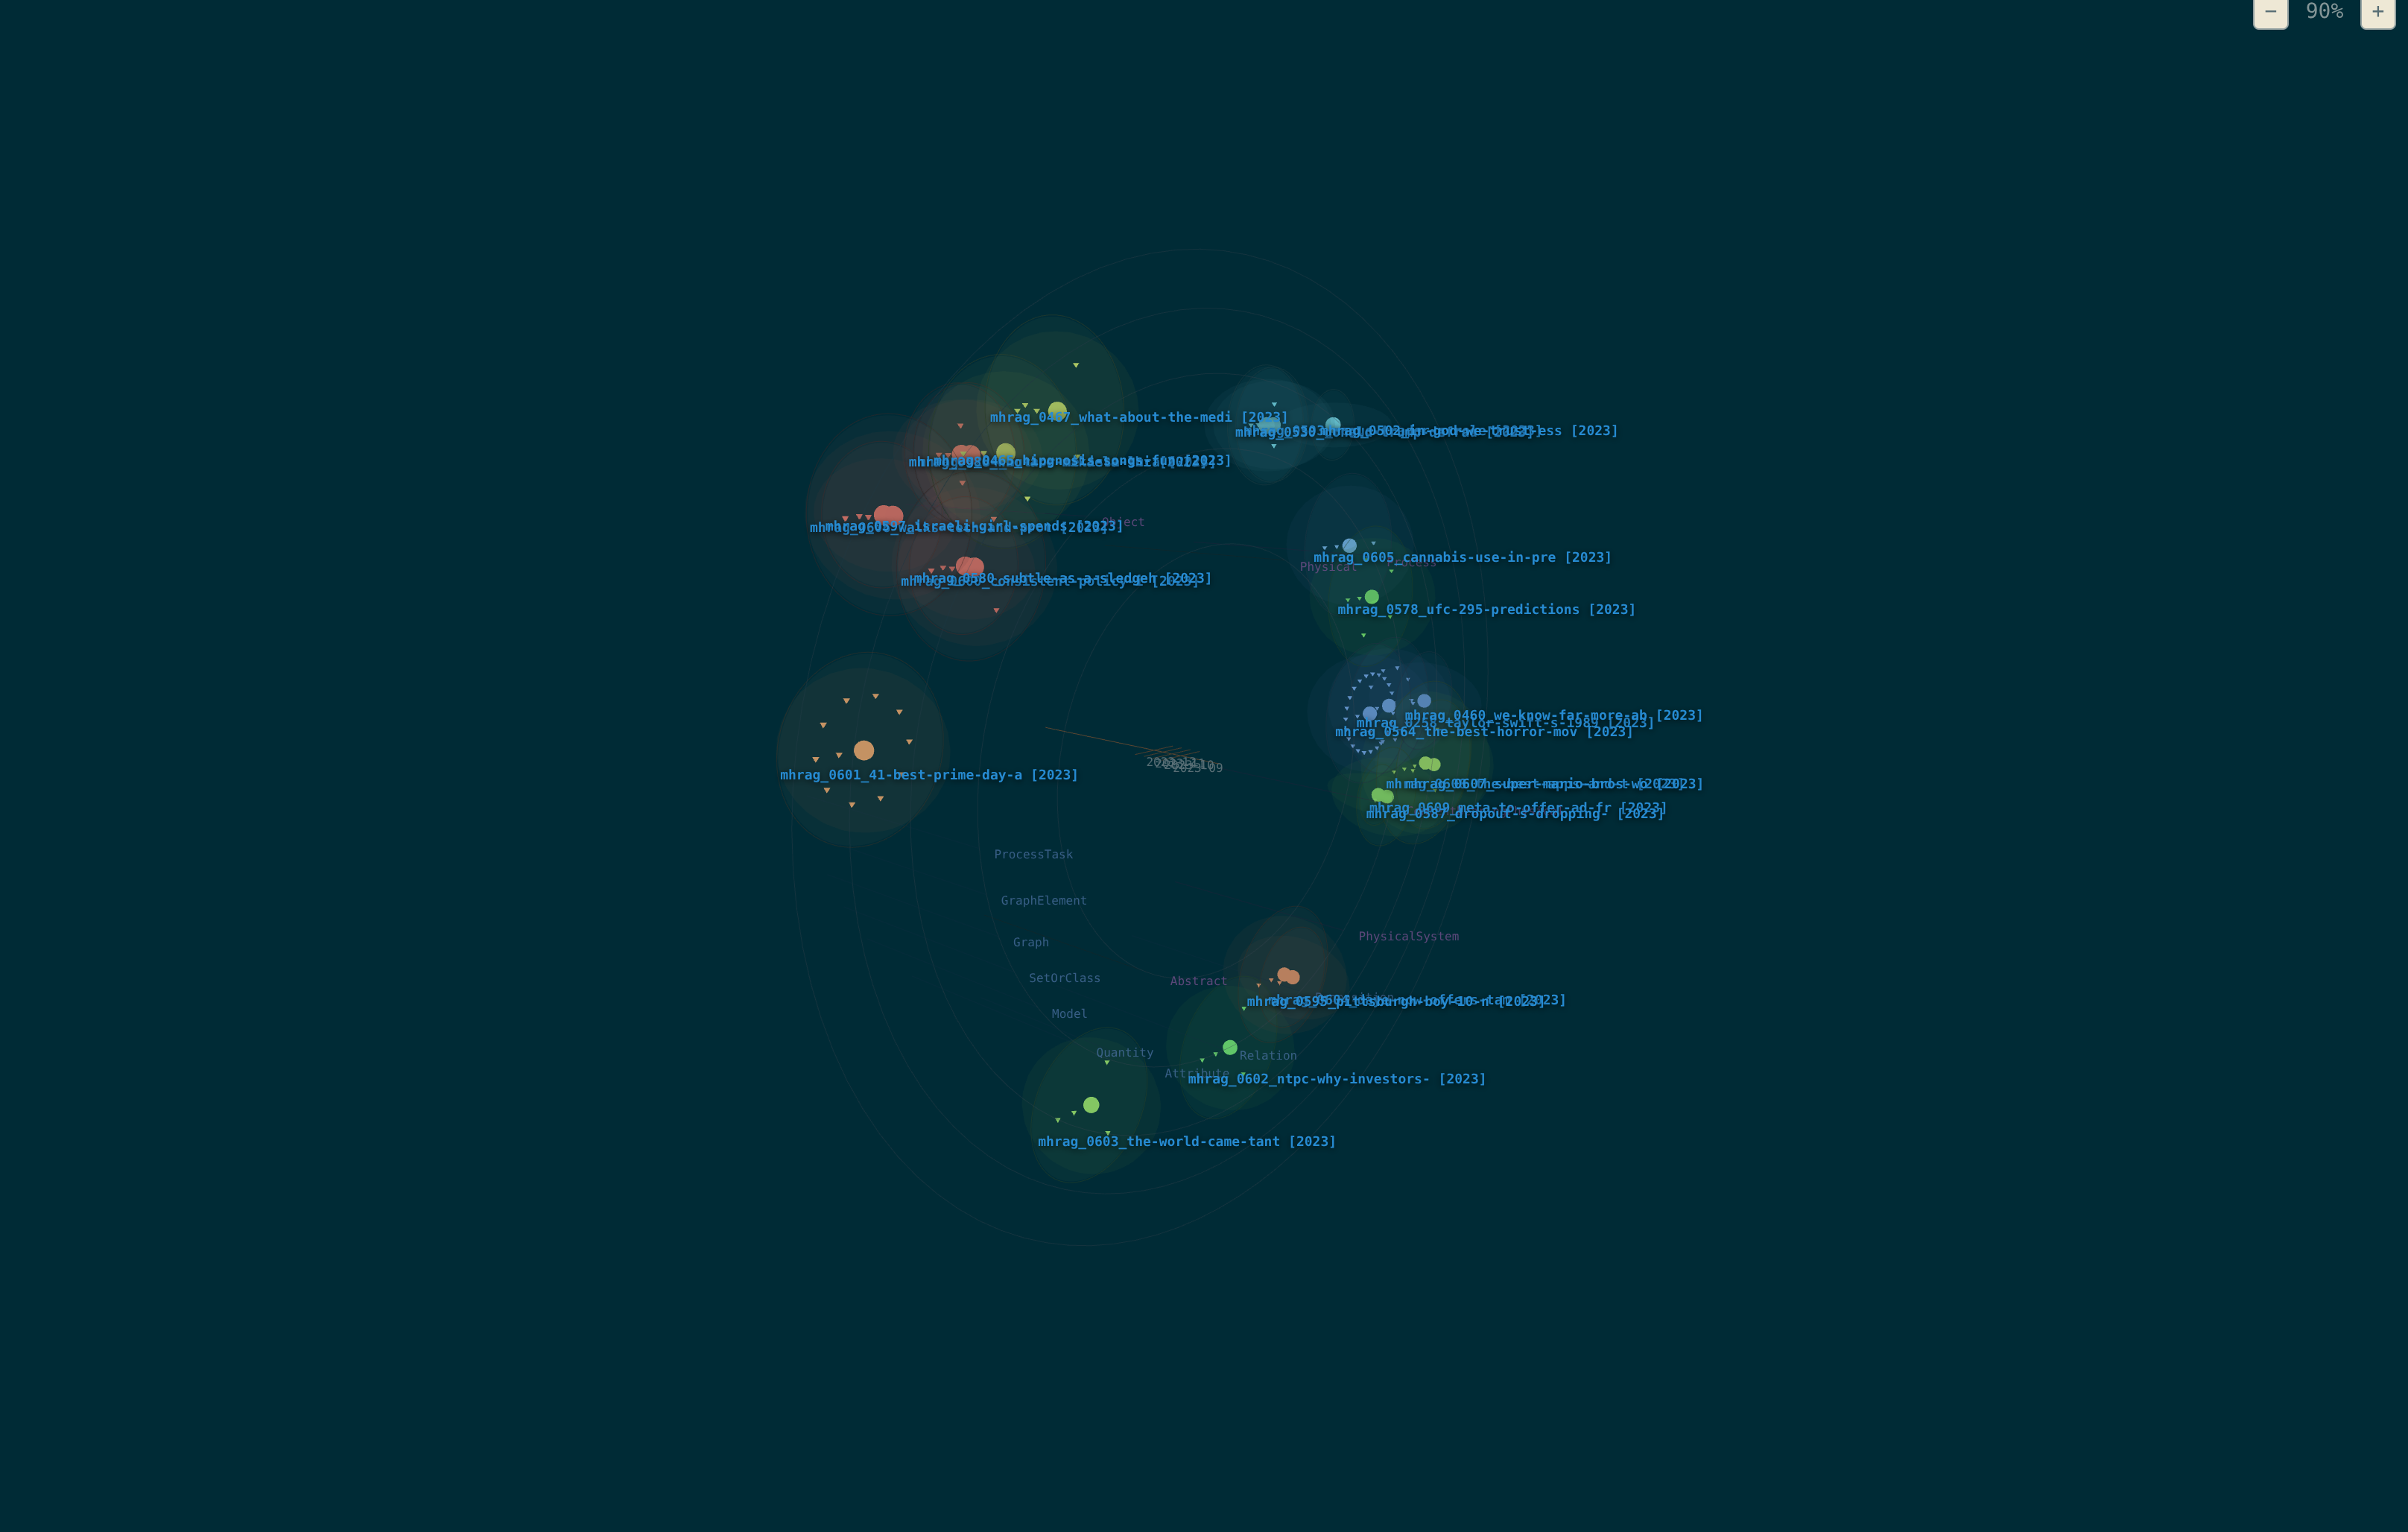
\includegraphics[width=0.48\columnwidth]{figs/tunnel_oblique.png}
\\[4pt]
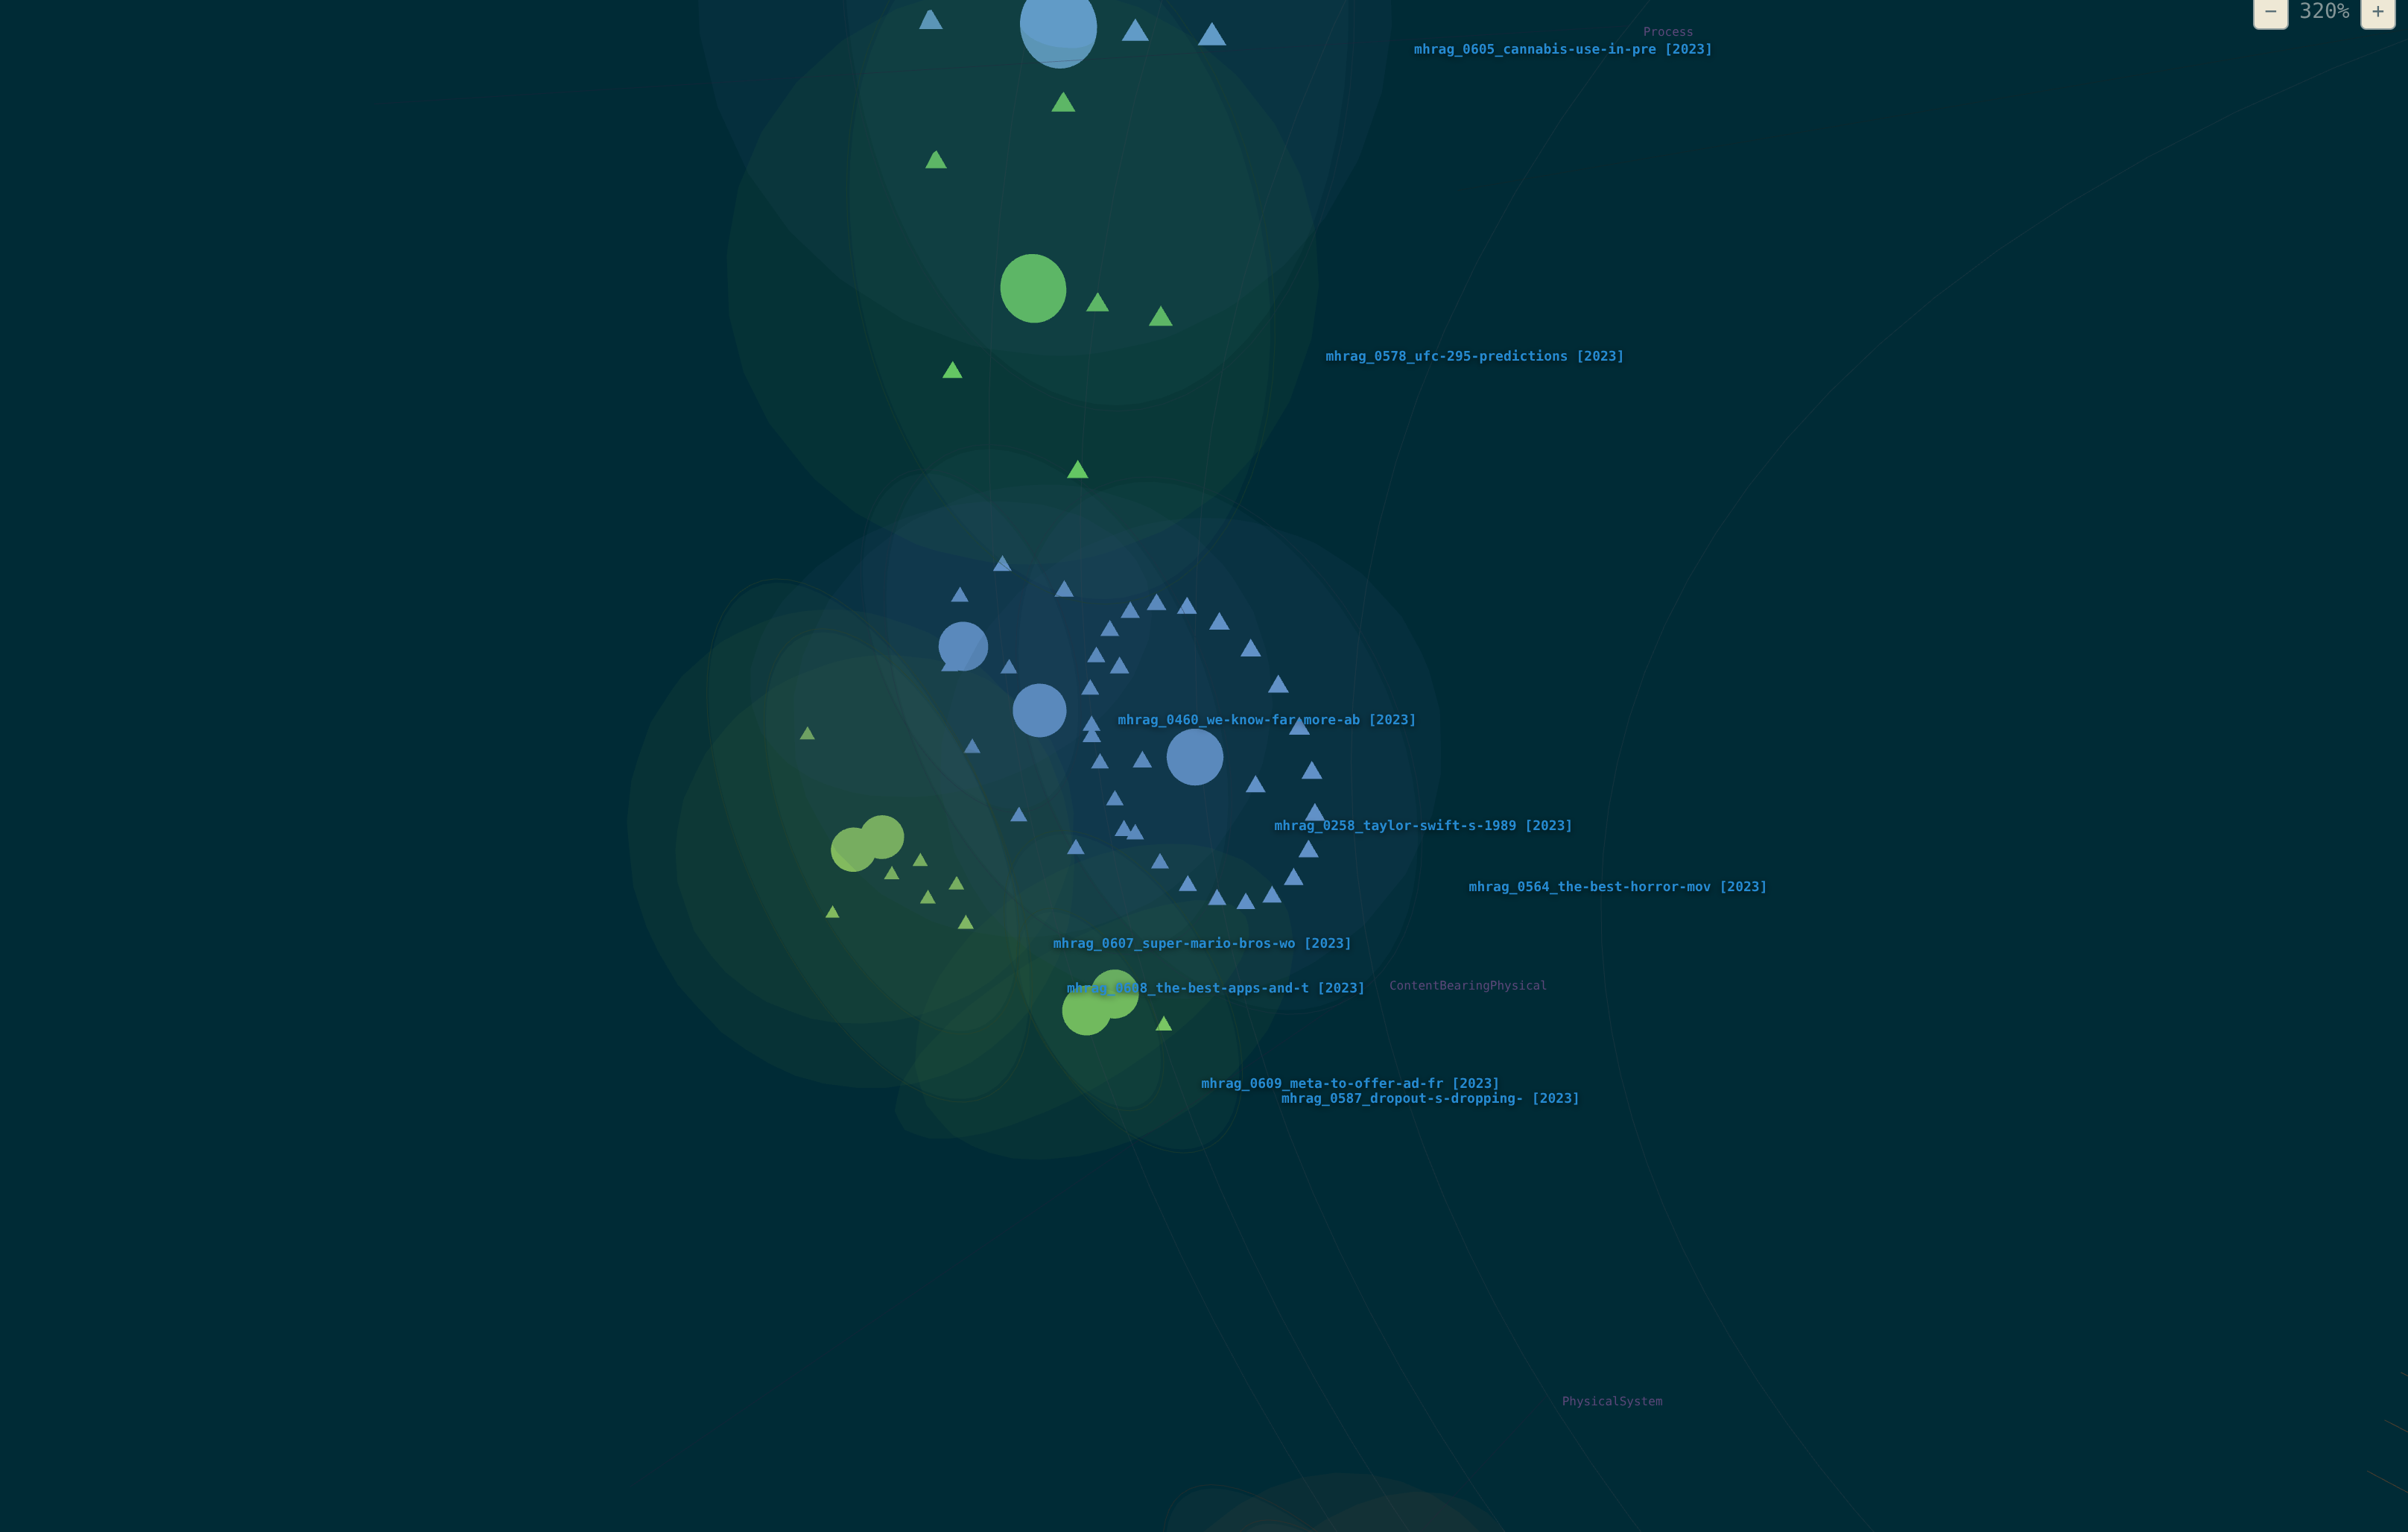
\includegraphics[width=0.7\columnwidth]{figs/disc_closeup.png}
\caption{Three camera views of the same 25-document Space-Time Graph (color = top SUMO category per document). \emph{Top left}: sunburst top-down, looking down $-$Y along the ontology cross-section -- documents cluster into SUMO category columns (\textit{Process}, \textit{Physical}, \textit{Object}, \textit{Proposition} labels visible). \emph{Top right}: oblique tunnel view, camera offset along Z so publication time reads as depth. \emph{Bottom}: close-up on a single document disc, showing its section hierarchy as a concentric ring of nodes (triangles) around the document root (sphere).}
\label{fig:viz}
\end{figure}

\section{Conclusion}

OHARA's Space-Time Graph unifies structural hierarchy, temporal decay, and ontology pivots into a single navigable substrate. The framework delivers retrieval performance at parity with dense vector baselines while establishing a corroboration-gated Principal tier that abstains on 45.6\% of unanswerable queries. Offline ingestion builds the complete semantic graph at $\sim$\$12 per 1{,}000 documents, and 3D rendering scales sub-linearly. In our point of view, these findings demonstrate that knowledge bases can be designed to be both humanly seeable and quantitatively auditable.

\section*{Acknowledgments}
This research is supported by research funding from University of Science, Vietnam National University -- Ho Chi Minh City.

\begin{thebibliography}{9}

\bibitem{liu2024lost}
N.~F. Liu, K.~Lin, J.~Hewitt, A.~Paranjape, M.~Bevilacqua, F.~Petroni, and P.~Liang, ``Lost in the middle: How language models use long contexts,'' \emph{Trans. Assoc. Comput. Linguist.}, vol.~12, pp.~157--173, 2024.

\bibitem{stasko2000focus}
J.~Stasko and E.~Zhang, ``Focus+context display and navigation techniques for enhancing radial, space-filling hierarchy visualizations,'' in \emph{Proc. IEEE InfoVis}, 2000, pp.~57--65.

\bibitem{tang2024multihop}
Y.~Tang and Y.~Yang, ``MultiHop-RAG: Benchmarking retrieval-augmented generation for multi-hop queries,'' arXiv:2401.15391, 2024.

\bibitem{dasigi2021qasper}
P.~Dasigi, K.~Lo, I.~Beltagy, A.~Cohan, N.~A. Smith, and M.~Gardner, ``A dataset of information-seeking questions and answers anchored in research papers,'' in \emph{Proc. NAACL}, 2021, pp.~4599--4610.

\bibitem{gao2023ragsurvey}
Y.~Gao, Y.~Xiong, X.~Gao, K.~Jia, J.~Pan, Y.~Bi, Y.~Dai, J.~Sun, Q.~Guo, M.~Wang, and H.~Wang, ``Retrieval-augmented generation for large language models: A survey,'' arXiv:2312.10997, 2023.

\bibitem{peng2024graphrag_survey}
B.~Peng, Y.~Zhu, Y.~Liu, X.~Bo, H.~Shi, C.~Hong, Y.~Zhang, and S.~Tang, ``Graph retrieval-augmented generation: A survey,'' arXiv:2408.08921, 2024.

\bibitem{edge2024graphrag}
D.~Edge, H.~Trinh, N.~Cheng, J.~Bradley, A.~Chao, A.~Mody, S.~Truitt, and J.~Larson, ``From local to global: A graph RAG approach to query-focused summarization,'' arXiv:2404.16130, 2024.

\bibitem{guo2024lightrag}
Z.~Guo, L.~Xia, Y.~Yu, T.~Ao, and C.~Huang, ``LightRAG: Simple and fast retrieval-augmented generation,'' arXiv:2410.05779, 2024.

\bibitem{gutierrez2024hipporag}
B.~J. Gutierrez, Y.~Shu, Y.~Gu, M.~Yasunaga, and Y.~Su, ``HippoRAG: Neurobiologically inspired long-term memory for large language models,'' in \emph{Proc. NeurIPS}, 2024.

\bibitem{asai2023selfrag}
A.~Asai, Z.~Wu, Y.~Wang, A.~Sil, and H.~Hajishirzi, ``Self-RAG: Learning to retrieve, generate, and critique through self-reflection,'' in \emph{Proc. ICLR}, 2024.

\bibitem{yan2024crag}
S.-Q. Yan, J.-C. Gu, Y.~Zhu, and Z.-H. Ling, ``Corrective retrieval augmented generation,'' arXiv:2401.15884, 2024.

\end{thebibliography}

\end{document}